%%%%%%%%%%%%%%%%%%%%%%%%%%%%%%%%%%%%%%%%%
% University/School Laboratory Report
% LaTeX Template
% Version 2.0 (4/12/12)
%
% This template has been downloaded from:
% http://www.latextemplates.com
%
% License:
% CC BY-NC-SA 3.0 (http://creativecommons.org/licenses/by-nc-sa/3.0/)
%
% Original header:
%
%
%%%%%%%%%%%%%%%%%%%%%%%%%%%%%%%%%%%%%%%%%

%----------------------------------------------------------------------------------------
%	DOCUMENT CONFIGURATIONS
%----------------------------------------------------------------------------------------

\documentclass{article}

\usepackage{graphicx} % Allows the inclusion of images

\title{General Approach for adding the \\ "Custom Importable Models" \\functionality} % Title

\author{Jonny \textsc{Quarta}} % Author name

\date{\today} % Specify a date for the report

\begin{document}

\maketitle % Insert the title, author and date


\setlength\parindent{0pt} % Removes all indentation from paragraphs

\renewcommand{\labelenumi}{\alph{enumi}.} % Make numbering in the enumerate environment by letter rather than number (e.g. section 6)



\section{Introduction}
Every neuronal simulator must provide an important number of different neuron models so that the user can choose which neuron type to instantiate from a large set, making the simulations more realistic. \\
The standard way this is achieved is by encapsulating these models inside the simulator itself using inheritance (where each model is described by a child class), or by describing them inside some sort of file, making the system more flexible. The second approach inspired the current work.\\
In order to make such a system as flexible as possible, some basic features have to be met:
\begin{itemize}
\item The user should write its own models in an easy way, using most of the knowledge he already has about programming.
\item The model integration into the system should be as flexible as possible.
\item The system should provide no difference in use between embedded and imported models.
\item The imported models should not lose to much performance compared to the embedded ones.
\end{itemize}
The purpose of this paper is to present a system like that, extrapolating the general principles required for its implementation and provide some concrete examples. \\



\section{General Approach}
The first question coming to mind usually is: what should the model description language look like?
The answer depends on several considerations, one of them being however dominant over the others: that language should be easy to use and known by as many people as possible. \\
These requirements are met by Python, which is widely used by the scientific community, both because of its easy utilization and for its powerfullness. \\
The following sections will describe the integration between Python and the NEST simulator, providing a concrete example of how such a system works. \\ \\

NEST has a Python interface, CyNEST, enabling the user to instantiate the neurons, set the experiment, simulate it and record the output data (for an overview, see \emph{http://www.nest-initiative.org/index.php/Software:About\_NEST} and \\ \emph{http://www.nest-initiative.org/index.php/PyNEST}). \\
In order to bind NEST and Python, Cython has been used. This tool provides a way for writing Python code (or even Cython code, which is an overset) and translate it into C or C++. This way, one can write the simulator core in C++ and the interface in Python, making it importable from a Python terminal. For an overview of Cython, see \emph{http://docs.cython.org}.\\ \\

One of the most interesting features of Cython is the \textbf{pyximport} module, which enables one to automatically compile and link cython code at runtime. This is done by writing:
\begin{verbatim}
import pyximport
pyximport.install()

import my_module #where my_module.pyx contains cython code
... 
# my_module is automatically compiled, linked and 
# is available to the code, just like in normal Python
\end{verbatim}

The general approach is therefore the following:
\begin{itemize}
\item Providing a function for model registration (in NEST is \emph{cynest.RegisterNeuron(...)}).
\item Inside that function, import (compile) the .pyx file containing the model.
\item Each time a custom neuron is instantiated, create the python object and give it to the C++ kernel as a PyObject (the kernel uses the Python/C library).
\item The kernel calls the different PyObject methods whenever needed (update, calibrate, etc... this depends on the simulator implementation).
\end{itemize}
This approach, when some important optimizations are carried out, turns out to be very time efficient, slowing down the system only up to 20-30\%, which is a good compromise when compared to the flexibility benefits.

\section{Proof of Concept by Example : CyNEST Structure}
This section seeks to demonstrate the faisability of the approach by describing the general structure of CyNEST itself. The figure depictes it:

\begin{figure}[h]
\begin{center}
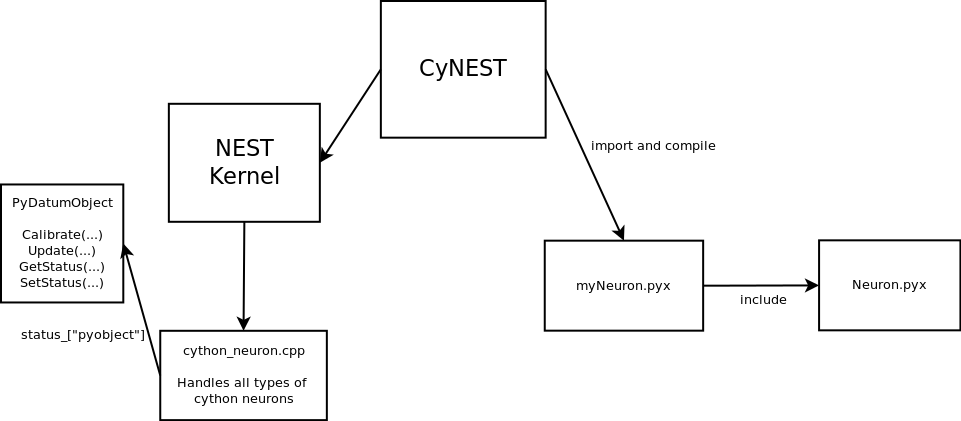
\includegraphics[width=0.92\textwidth]{Ressources/CyNEST_Structure}
\caption{CyNEST Structure}
\end{center}
\end{figure}
As one can see, the CyNEST module is at the top of the hierarchy. On one hand, it can import the different models (using pyximport) and on the other hand, it has access to the NEST simulator (for a review on how to include C++ code into a cython project please consult the official documentation), which will be called for every operation on the kernel (adding new neurons to the network, simulating, setting parameters, etc...). \\
Note that the .pyx file must contain the class definition of the custom model (see next section for more details).\\
The key idea is that whenever the user instantiates a neuron of an imported type, CyNEST will create an instance of the model class and give it to the kernel as a PyObject. The latter will then call the different methods using the Python/C library.

\section{Custom Model Structure}
This section aims to present a possible model structure. This is by no means the only implementable one, but has the advantage of being particularly easy and well suitable for integration with NEST.\\
The minimal code for writing a new model is the following:
\begin{verbatim}
include "[NEST installation path]/include/Neuron.pyx"

cdef class sample_neuron(Neuron):
    cdef int param1
    ...

    def __cinit__(self):
        self.param1 = ...
        ...

    cpdef calibrate(self):
        ...

    cpdef update(self):
        ...

    cpdef getStatus(self):
        cdef dict d = {}

        d["param1"] = self.param
        ...
        return d

    cpdef setStatus(self, d):
        if "param1" in d:
            self.param1 = d["param1"]
        ...

\end{verbatim}
Each new model is represented by a class extending from a base Neuron parent, which is contained in a special file located at \emph{[NEST installation path]/include/Neuron.pyx}.
As one can see, the child class has to overwrite a certain amount of functions, which will be called instead of the normal embedded neuron methods.\\
This approach has the advantage of letting the user using Python objects or functions inside the neuron.


\section{Optimizations}
In order to make the system as fast as possible, a few considerations have to be carried out.\\ \\
The first one is about the neuron parameters. In order to be callable, a parameter must be located inside the cython class (making a \emph{cdef ...}, however if the user wants to see the neuron attribute values, for example after a simulation, they have to be available to the NEST kernel, inside some status dictionary. This is done by translating them during the \emph{SetStatus} and \emph{GetStatus} methods. \\
Now, the real point is that this is fine when dealing with user operations, but doesn't work when dealing with simulations. Before the \emph{Update} method is called, the kernel has to update some neuron parameters (for example, the incoming spikes), which means that these new values have to be "manually" updated inside the neuron model by first converting them, which is far too slow. \\
The solution is to extract the pointers so that the kernel has direct access to the variable location. Of course this works easily only with primitive types. As an example, let's take the extraction of the \emph{incoming spikes} parameter:
\begin{verbatim}
Neuron.pyx:
    ...
    def getIn_SpikesPointer():
        return <long>(&(self.in_spikes))
\end{verbatim}
On the kernel side, we can call this method by writing:
\begin{verbatim}
in_spikes = PyInt_AsLong(PyObject_CallMethod(this->pyObj, "getIn_SpikesPointer", NULL));
\end{verbatim}
Now, the \emph{in\_spikes} is available from the two sides without any conversion and the result is much faster (factor of 3).\\ \\

A second consideration involves the Python/C method calling convension. As one could expect, it is very slow, but can be significantly improved by extracting the direct function pointer. This is very important only with the \emph{Update} method, because it is always called during a simulation.
In order to extract a function pointer, one has to write:
\begin{verbatim}
PyMethodDef *tp_methods = this->pyObj->ob_type->tp_methods
PyMethodDef *updateRef = NULL;

int i = 0;
while(&(tp_methods[i]) != NULL) {
    if(std::string("update").compare(tp_methods[i].ml_name) == 0) {
        updateRef = &(tp_methods[i]);
    }
    i++;
}

PyCFunction updateFct = updateRef->ml_meth;
\end{verbatim}
The list of the different methods is contained in the \emph{PyObject::ob\_type::tp\_methods} array. The loop seeks for the update method and iterates until the next array element is NULL. Finally, when the \emph{PyMethodDef} structure corresponding to the update method is found, the \emph{PyMethodDef::ml\_meth} attribute extracts a \emph{PyCFunction} element, which is just the callable function pointer.\\
Directly calling the function pointer speeds a lot the simulation (a factor of 2).


\section{Accessing Kernel Objects from the Model}
It is sometimes useful to make kernel objects available from the model side. It is important for example when dealing with specific simulation parameters, such as the time between two simulation steps, etc...\\
The problem is that using pyximport the .pyx file has no access to the calling project and cannot therefore see class definitions. Is there a way to avoid this problem? Luckily, there is.\\
If the .pyx file contains the definition of a general object, then it is possible for the base project to fill this element with whatever python object he wants. Here is an example:
\begin{verbatim}
.pyx file:
    ...
    cdef class ObjectManager:
        cdef object myObj
        ...

        def setObject(self, obj):
            self.myObj = obj
        ...

    cdef ObjectManager objectManager = ObjectManager()


# These methods are called from the project 

    def setObject(obj):
        objectManager.setObject(obj)
    ...


project side:
    exec(pyx_file_name + ".setObject(obj)")
\end{verbatim}
Note that the .pyx file structure is very important. If for example \emph{myObj} were declared global and filled from the project side, then on the .pyx file side it would be NULL. However, by englobing it in an object instantiated inside the .pyx file, no problem occurs.\\ \\

Now that we have project objects available, we want to instantiate many of them (we only have one until now). The trick is to provide each one of these objects with a special \emph{create} method returning a new instance.


\section{Performances}
The system has been tested during a single-threaded simulation of 40 ms concerning over 1000 randomly connected neurons and compared to their native (embedded models) counterparts. The results are:
\begin{itemize}
\item Native neuron: realtime factor is 0.3254
\item Cython neuron: realtime factor is 0.2711
\end{itemize}
We can therefore conclude that the cython neuron is only about 20\% slower than the native version.
Note that during different test trials, values could slightly change because of the random factor introduced in the network.


\section{Conclusion}

\end{document}